\subsection*{Running Time of Disjoint Set}

We now show that the above balancing procedure guarantees
that, the height of any tree is $\Theta(\log n)$. 
\begin{fact}
Let $T$ be a tree with $n$ nodes. Then $h(T) \le 1 + \log_2 n$, where $h(T)$ denotes the height of $T$.
\end{fact}
\emph{Proof.} The \emph{make-set} creates a new tree with a single node, and clearly it holds above fact.
The \emph{find} operation queries but doesn't change anything. We now show the \emph{union}
holds above fact too. We prove it by induction: suppose the before merging $T_1$ and $T_2$
with $n_1$ and $n_2$ nodes respectively, we have $h(T_1) \le 1 + \log n_1$ and $h(T_2) \le 1 + \log n_2$.
Note that after mering we have $n = n_1 + n_2$.
Consider the 3 cases in the union procedure. 
If $h(T_1) < h(T_2)$, then $h(T) = h(T_2) \le 1 + \log n_2 \le 1 + \log n$, as desired.
The same for $h(T_1) > h(T_2)$. Now consider $h(T_1) = h(T_2)$.
In this case $h(T) = h(T_1) + 1 = h(T_2) + 1$.
We can write $2h(T) = 2 + h(T_1) + h(T_2) \le 4 + \log n_1 + \log n_2 = 4 + \log n_1n_2 \le 4 + \log((n_1+n_2)/2)^2 = 4 + 2\log (n/2) = 2(1+\log n)$,
   which gives the desired $h(T) \le 1 + \log n$.  \qed

Hence, the \emph{make-set} takes $\Theta(1)$ time.
The \emph{find} takes $\Theta(\log n)$ time.
The \emph{union} takes $\Theta(\log n)$ time as well; it is dominated by the \emph{find} procedure; the remaining of \emph{union}
after calling find takes $\Theta(1)$ time.

\subsection*{Complete Kruskal's Algorithm}

Recall that, at any time of the Kruskal's algorithm, the vertices are implicitly
partitioned
into a collection of connected components by $E_1$,
and adding an edge $e = (u,v)$ to $E_1$ doesn't produce a cycle
if and only if $u$ and $v$ are in different components.
Hence, we can use a disjoint-set data structure
to maintain the connected components formed by $E_1$, 
where each set here corresponds to a component.
Determining whether adding an edge $e=(u,v)$ leads to a cycle 
is equivalent to determining if $u$ and $v$ are in the same component,
which can be answered by querying if $find(u)$ equals to $find(v)$.
If $find(u)$ is not equal to $find(v)$, then $e$ can be safely added.
Adding $e$ results in the merging the two connected components~(containing $u$ and $v$ respectively);
we can then simply call $union(u,v)$ to update the
disjoint-set to reflect the merging.
The complete algorithm is given below.

\begin{algorithmblock}[0.8\textwidth]
	\aaA {11}{Algorithm Kruskal's~($G = (V,E), w(e) \forall e\in E$)}\xxx
	\aab {sort all edges in $E$ by weights in ascending order;}\xxx
	\aab {$E_1 = \emptyset$;}\xxx
	\aab {for each $v\in V$: call \emph{make-set~($v$)}; \ // as $E_1 = \emptyset$, each vertex forms a set of its own}\xxx
	\aaB {6}{for each $e = (u,v)\in E$ following above ordering}\xxx
	\aac {$r_u = find(u)$}\xxx
	\aac {$r_v = find(v)$}\xxx
	\aaC {3}{if~($r_u\neq r_v$)}\xxx
	\aad {$E_1 = E_1\cup \{e\}$}\xxx
	\aad {$union(r_u,r_v)$}\xxx
\end{algorithmblock}

Sorting takes $\Theta(|E|\log|E|) = \Theta(|E|\log|V|)$ time~(note that $\log |E| \le \log |V|^2 = 2\log |V|$).
Examining all edges takes $\Theta(|E|\log|V|)$ too.
So the entire algorithm runs in $\Theta(|E|\log|V|)$ time.


\subsection*{Complete Prim's Algorithm}

Recall that the Prim's algorithm maintains a single connected component $S$.
$S$ is initialized with an arbitrarily picked vertex, and in each iteration,
the algorithm picks an edge with minimized weight that connects $S$ to a \emph{new} vertex outside $S$.
In other words, in each iteration, the algorithm picks the smallest cut-edge w.r.t.\ cut $(S, V\setminus S)$,
formally written as $\arg\min_{e=(u,v), u\in S, v\not\in S} w(e)$.
An efficient implementation requires a data structure that can quickly compute the minimization.

We use \emph{priority queue}.
In a priority queue, each element is labeled with a \emph{priority}~(also called key).
%The priority/key serves as the identify of the element.
%In other words, each element in a priority queue is a pair (\emph{key, value}),
%where \emph{key} indicates its priority, while \emph{value} stores the actual data.
A {priority queue} data structure supports the following operations.
\begin{enumerate}
\item empty~($PQ$): decides if priority queue $PQ$ is empty;
\item insert~($PQ$, $x$, \emph{key}): add element $x$ to $PQ$ with priority being \emph{key};
\item find-min~($PQ$): return the element in $PQ$ with smallest key~(i.e., highest priority);
\item delete-min~($PQ$): remove the element in $PQ$ with smallest key~(i.e., highest priority).
\item decrease-key~($PQ$, $x$, \emph{new-key}): set the key of the specified element $x$ as the given \emph{new-key}.
\end{enumerate}

The major advantage of the priority queue is that find-min can be done quickly.
With a binary heap implementation, the above 5 operations takes $O(1)$, $O(\log n)$, $O(1)$,
$O(\log n)$, and $O(\log n)$ time, respectively.

Throughout the Prim's algorithm, we use priority queque $PQ$ to store $V\setminus S$, i.e., 
the vertices that are not yet added to $S$.
(Hence, implicitly maintaining $S$ is not needed, as it is complement to $PQ$.)
Now think: what the priority/key of a vertex in $PQ$ should be?
The priority/key of a vertex $v$ in $PQ$~(i.e., in $V\setminus S$) 
should be the weight of the smallest edge that connects $S$ to $v$, formally written as
$key[v] := \min_{e=(u,v), u\in S} w(e)$.
This works because, \emph{find-min~($PQ$)} gives
$\min_{v\not\in S} key[v] = \min_{e=(u,v), u\in S, v\not\in S} w(e)$, which is exactly 
the weight of the smallest cut-edge. % w.r.t.\ cut $(S,V\setminus S)$.
Another way to understand it is that, cut-edges are grouped according to their ends in $V\setminus S$;
finding the smallest cut-edge is done in two steps: the first step finds the smallest edge in each group,
i.e., $\min_{e=(u,v), u\in S} w(e)$,  for each $v\in V\setminus S$, 
which is defined as the priority/key of $v$;
the second step finds the smallest edge across groups, i.e., $\min_{v\in V\setminus S} key[v]$.
See  Figure~\ref{fig:prim} for an example.

\begin{figure}[h]
\centering{

\tikzset{every picture/.style={line width=0.75pt}} %set default line width to 0.75pt        

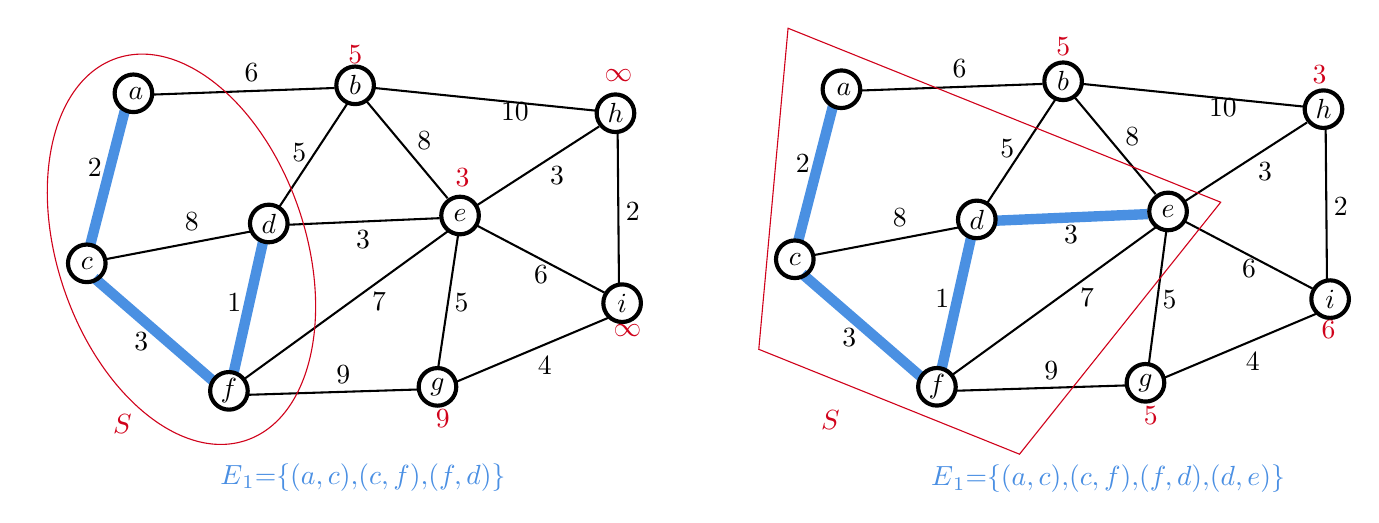
\begin{tikzpicture}[x=0.48pt,y=0.48pt,yscale=-1,xscale=1]
%uncomment if require: \path (0,459); %set diagram left start at 0, and has height of 459

%Straight Lines [id:da6278329343253372] 
\draw [color={rgb, 255:red, 0; green, 0; blue, 0 }  ,draw opacity=1 ][line width=0.75]    (269,67) -- (330,140) ;
%Straight Lines [id:da9826257751124597] 
\draw [color={rgb, 255:red, 0; green, 0; blue, 0 }  ,draw opacity=1 ][line width=0.75]    (179,288) -- (307,284) ;
%Straight Lines [id:da9824647104655378] 
\draw [color={rgb, 255:red, 74; green, 144; blue, 226 }  ,draw opacity=1 ][line width=3.75]    (64,200) -- (154,278) ;
%Straight Lines [id:da5609469664096045] 
\draw [color={rgb, 255:red, 0; green, 0; blue, 0 }  ,draw opacity=1 ][line width=0.75]    (72,186) -- (182,165) ;
%Straight Lines [id:da866584153602073] 
\draw [color={rgb, 255:red, 74; green, 144; blue, 226 }  ,draw opacity=1 ][line width=3.75]    (87,74) -- (61,175) ;
%Straight Lines [id:da8429173178729373] 
\draw [color={rgb, 255:red, 0; green, 0; blue, 0 }  ,draw opacity=1 ][line width=0.75]    (107,62) -- (245,57) ;
%Straight Lines [id:da20128821894816062] 
\draw [color={rgb, 255:red, 0; green, 0; blue, 0 }  ,draw opacity=1 ][line width=0.75]    (255,68) -- (203,147) ;
%Straight Lines [id:da4356587454282608] 
\draw [color={rgb, 255:red, 74; green, 144; blue, 226 }  ,draw opacity=1 ][line width=3.75]    (191,173) -- (169,271) ;
%Straight Lines [id:da14466126019097159] 
\draw [color={rgb, 255:red, 0; green, 0; blue, 0 }  ,draw opacity=1 ][line width=0.75]    (330,165) -- (177,276) ;
%Straight Lines [id:da2637375879467664] 
\draw [color={rgb, 255:red, 0; green, 0; blue, 0 }  ,draw opacity=1 ][line width=0.75]    (324,155) -- (209,160) ;
%Shape: Ellipse [id:dp04172567316274278] 
\draw  [color={rgb, 255:red, 208; green, 2; blue, 27 }  ,draw opacity=1 ] (41.23,208.4) .. controls (14.29,128.98) and (32.03,51.17) .. (80.86,34.61) .. controls (129.7,18.04) and (191.12,68.99) .. (218.07,148.41) .. controls (245.01,227.83) and (227.27,305.64) .. (178.44,322.21) .. controls (129.6,338.78) and (68.18,287.82) .. (41.23,208.4) -- cycle ;
%Straight Lines [id:da22995917519031528] 
\draw [color={rgb, 255:red, 0; green, 0; blue, 0 }  ,draw opacity=1 ][line width=0.75]    (275,57) -- (441,74) ;
%Straight Lines [id:da5296708685106871] 
\draw [color={rgb, 255:red, 0; green, 0; blue, 0 }  ,draw opacity=1 ][line width=0.75]    (458,89) -- (459,204) ;
%Straight Lines [id:da7230804292624167] 
\draw [color={rgb, 255:red, 0; green, 0; blue, 0 }  ,draw opacity=1 ][line width=0.75]    (444,86) -- (351,146) ;
%Straight Lines [id:da9640499330506606] 
\draw [color={rgb, 255:red, 0; green, 0; blue, 0 }  ,draw opacity=1 ][line width=0.75]    (351,160) -- (448,211) ;
%Straight Lines [id:da1957235990181826] 
\draw [color={rgb, 255:red, 0; green, 0; blue, 0 }  ,draw opacity=1 ][line width=0.75]    (451,230) -- (337,278) ;
%Straight Lines [id:da11647241183092005] 
\draw [color={rgb, 255:red, 0; green, 0; blue, 0 }  ,draw opacity=1 ][line width=0.75]    (802,63.94) -- (863,136.94) ;
%Straight Lines [id:da31981297939132225] 
\draw [color={rgb, 255:red, 0; green, 0; blue, 0 }  ,draw opacity=1 ][line width=0.75]    (712,284.94) -- (840,280.94) ;
%Straight Lines [id:da7983678270493085] 
\draw [color={rgb, 255:red, 74; green, 144; blue, 226 }  ,draw opacity=1 ][line width=3.75]    (597,196.94) -- (687,274.94) ;
%Straight Lines [id:da3869238966612649] 
\draw [color={rgb, 255:red, 0; green, 0; blue, 0 }  ,draw opacity=1 ][line width=0.75]    (605,182.94) -- (715,161.94) ;
%Straight Lines [id:da32951243577855704] 
\draw [color={rgb, 255:red, 74; green, 144; blue, 226 }  ,draw opacity=1 ][line width=3.75]    (620,70.94) -- (594,171.94) ;
%Straight Lines [id:da948271107244244] 
\draw [color={rgb, 255:red, 0; green, 0; blue, 0 }  ,draw opacity=1 ][line width=0.75]    (640,58.94) -- (778,53.94) ;
%Straight Lines [id:da9060839913160768] 
\draw [color={rgb, 255:red, 0; green, 0; blue, 0 }  ,draw opacity=1 ][line width=0.75]    (788,64.94) -- (736,143.94) ;
%Straight Lines [id:da54757624583718] 
\draw [color={rgb, 255:red, 74; green, 144; blue, 226 }  ,draw opacity=1 ][line width=3.75]    (724,169.94) -- (702,267.94) ;
%Straight Lines [id:da3064468870257864] 
\draw [color={rgb, 255:red, 0; green, 0; blue, 0 }  ,draw opacity=1 ][line width=0.75]    (863,161.94) -- (710,272.94) ;
%Straight Lines [id:da27846949014065103] 
\draw [color={rgb, 255:red, 74; green, 144; blue, 226 }  ,draw opacity=1 ][line width=3.75]    (857,151.94) -- (742,156.94) ;
%Straight Lines [id:da23340445530829934] 
\draw [color={rgb, 255:red, 0; green, 0; blue, 0 }  ,draw opacity=1 ][line width=0.75]    (808,53.94) -- (974,70.94) ;
%Straight Lines [id:da19179449082275934] 
\draw [color={rgb, 255:red, 0; green, 0; blue, 0 }  ,draw opacity=1 ][line width=0.75]    (991,85.94) -- (992,200.94) ;
%Straight Lines [id:da4737172365295894] 
\draw [color={rgb, 255:red, 0; green, 0; blue, 0 }  ,draw opacity=1 ][line width=0.75]    (977,82.94) -- (884,142.94) ;
%Straight Lines [id:da33516212941033763] 
\draw [color={rgb, 255:red, 0; green, 0; blue, 0 }  ,draw opacity=1 ][line width=0.75]    (884,156.94) -- (981,207.94) ;
%Straight Lines [id:da6079537599641894] 
\draw [color={rgb, 255:red, 0; green, 0; blue, 0 }  ,draw opacity=1 ][line width=0.75]    (984,226.94) -- (870,274.94) ;
%Straight Lines [id:da15519763368476547] 
\draw [color={rgb, 255:red, 0; green, 0; blue, 0 }  ,draw opacity=1 ][line width=0.75]    (338,167) -- (323,267) ;
%Straight Lines [id:da7888476116503551] 
\draw [color={rgb, 255:red, 0; green, 0; blue, 0 }  ,draw opacity=1 ][line width=0.75]    (871,165) -- (858,264) ;
%Shape: Trapezoid [id:dp6408521319989767] 
\draw  [color={rgb, 255:red, 208; green, 2; blue, 27 }  ,draw opacity=1 ] (912,143) -- (760.54,332.67) -- (564.26,253.72) -- (586.31,12.01) -- cycle ;

% Text Node
\draw  [line width=1.5]   (339.38, 153) circle [x radius= 14.15, y radius= 14.15]   ;
\draw (339.38,153) node   [align=left] {$\displaystyle e$};
% Text Node
\draw  [line width=1.5]   (93.48, 61) circle [x radius= 14.15, y radius= 14.15]   ;
\draw (87.98,61) node [anchor=west] [inner sep=0.75pt]   [align=left] {$\displaystyle a$};
% Text Node
\draw  [line width=1.5]   (260.38, 55) circle [x radius= 14.15, y radius= 14.15]   ;
\draw (260.38,55) node   [align=left] {$\displaystyle b$};
% Text Node
\draw  [line width=1.5]   (58.38, 189) circle [x radius= 14.15, y radius= 14.15]   ;
\draw (58.38,189) node   [align=left] {$\displaystyle c$};
% Text Node
\draw  [line width=1.5]   (195.38, 159) circle [x radius= 14.15, y radius= 14.15]   ;
\draw (195.38,159) node   [align=left] {$\displaystyle d$};
% Text Node
\draw  [line width=1.5]   (165.38, 285) circle [x radius= 14.15, y radius= 14.15]   ;
\draw (165.38,285) node   [align=left] {$\displaystyle f$};
% Text Node
\draw  [line width=1.5]   (322.38, 282) circle [x radius= 14.15, y radius= 14.15]   ;
\draw (322.38,282) node   [align=left] {$\displaystyle g$};
% Text Node
\draw (57.24,108.06) node [anchor=north west][inner sep=0.75pt]   [align=left] {$\displaystyle 2$};
% Text Node
\draw (175.24,37.06) node [anchor=north west][inner sep=0.75pt]   [align=left] {$\displaystyle 6$};
% Text Node
\draw (259.24,162.06) node [anchor=north west][inner sep=0.75pt]   [align=left] {$\displaystyle 3$};
% Text Node
\draw (211.24,97.06) node [anchor=north west][inner sep=0.75pt]   [align=left] {$\displaystyle 5$};
% Text Node
\draw (130.24,149.06) node [anchor=north west][inner sep=0.75pt]   [align=left] {$\displaystyle 8$};
% Text Node
\draw (92.24,239.06) node [anchor=north west][inner sep=0.75pt]   [align=left] {$\displaystyle 3$};
% Text Node
\draw (162.24,210.06) node [anchor=north west][inner sep=0.75pt]   [align=left] {$\displaystyle 1$};
% Text Node
\draw (305.24,88.06) node [anchor=north west][inner sep=0.75pt]   [align=left] {$\displaystyle 8$};
% Text Node
\draw (244.24,264.06) node [anchor=north west][inner sep=0.75pt]   [align=left] {$\displaystyle 9$};
% Text Node
\draw (271.24,209) node [anchor=north west][inner sep=0.75pt]   [align=left] {$\displaystyle 7$};
% Text Node
\draw (157,338) node [anchor=north west][inner sep=0.75pt]   [align=left] {$\displaystyle \textcolor[rgb]{0.29,0.56,0.89}{E}\textcolor[rgb]{0.29,0.56,0.89}{_{1}}\textcolor[rgb]{0.29,0.56,0.89}{=}\textcolor[rgb]{0.29,0.56,0.89}{\{}\textcolor[rgb]{0.29,0.56,0.89}{(}\textcolor[rgb]{0.29,0.56,0.89}{a,c}\textcolor[rgb]{0.29,0.56,0.89}{)}\textcolor[rgb]{0.29,0.56,0.89}{,}\textcolor[rgb]{0.29,0.56,0.89}{(}\textcolor[rgb]{0.29,0.56,0.89}{c,f}\textcolor[rgb]{0.29,0.56,0.89}{)}\textcolor[rgb]{0.29,0.56,0.89}{,}\textcolor[rgb]{0.29,0.56,0.89}{(}\textcolor[rgb]{0.29,0.56,0.89}{f,d}\textcolor[rgb]{0.29,0.56,0.89}{)}\textcolor[rgb]{0.29,0.56,0.89}{\}}$};
% Text Node
\draw (76.24,301.06) node [anchor=north west][inner sep=0.75pt]   [align=left] {$\displaystyle \textcolor[rgb]{0.82,0.01,0.11}{S}$};
% Text Node
\draw  [line width=1.5]   (456.38, 76) circle [x radius= 14.15, y radius= 14.15]   ;
\draw (456.38,76) node   [align=left] {$\displaystyle h$};
% Text Node
\draw  [line width=1.5]   (461.38, 219) circle [x radius= 14.15, y radius= 14.15]   ;
\draw (461.38,219) node   [align=left] {$\displaystyle i$};
% Text Node
\draw (393.24,189) node [anchor=north west][inner sep=0.75pt]   [align=left] {$\displaystyle 6$};
% Text Node
\draw (368.24,66) node [anchor=north west][inner sep=0.75pt]   [align=left] {$\displaystyle 10$};
% Text Node
\draw (405.24,114) node [anchor=north west][inner sep=0.75pt]   [align=left] {$\displaystyle 3$};
% Text Node
\draw (462.24,141) node [anchor=north west][inner sep=0.75pt]   [align=left] {$\displaystyle 2$};
% Text Node
\draw (396,257) node [anchor=north west][inner sep=0.75pt]   [align=left] {$\displaystyle 4$};
% Text Node
\draw (253.24,23.06) node [anchor=north west][inner sep=0.75pt]  [color={rgb, 255:red, 208; green, 2; blue, 27 }  ,opacity=1 ] [align=left] {$\displaystyle 5$};
% Text Node
\draw (334,116) node [anchor=north west][inner sep=0.75pt]  [color={rgb, 255:red, 208; green, 2; blue, 27 }  ,opacity=1 ] [align=left] {$\displaystyle 3$};
% Text Node
\draw (319.24,297) node [anchor=north west][inner sep=0.75pt]  [color={rgb, 255:red, 208; green, 2; blue, 27 }  ,opacity=1 ] [align=left] {$\displaystyle 9$};
% Text Node
\draw (453,233) node [anchor=north west][inner sep=0.75pt]  [color={rgb, 255:red, 208; green, 2; blue, 27 }  ,opacity=1 ] [align=left] {$\displaystyle \infty $};
% Text Node
\draw (446.24,41) node [anchor=north west][inner sep=0.75pt]  [color={rgb, 255:red, 208; green, 2; blue, 27 }  ,opacity=1 ] [align=left] {$\displaystyle \infty $};
% Text Node
\draw  [line width=1.5]   (872.38, 149.94) circle [x radius= 14.15, y radius= 14.15]   ;
\draw (872.38,149.94) node   [align=left] {$\displaystyle e$};
% Text Node
\draw  [line width=1.5]   (626.48, 57.94) circle [x radius= 14.15, y radius= 14.15]   ;
\draw (620.98,57.94) node [anchor=west] [inner sep=0.75pt]   [align=left] {$\displaystyle a$};
% Text Node
\draw  [line width=1.5]   (793.38, 51.94) circle [x radius= 14.15, y radius= 14.15]   ;
\draw (793.38,51.94) node   [align=left] {$\displaystyle b$};
% Text Node
\draw  [line width=1.5]   (591.38, 185.94) circle [x radius= 14.15, y radius= 14.15]   ;
\draw (591.38,185.94) node   [align=left] {$\displaystyle c$};
% Text Node
\draw  [line width=1.5]   (728.38, 155.94) circle [x radius= 14.15, y radius= 14.15]   ;
\draw (728.38,155.94) node   [align=left] {$\displaystyle d$};
% Text Node
\draw  [line width=1.5]   (698.38, 281.94) circle [x radius= 14.15, y radius= 14.15]   ;
\draw (698.38,281.94) node   [align=left] {$\displaystyle f$};
% Text Node
\draw  [line width=1.5]   (855.38, 278.94) circle [x radius= 14.15, y radius= 14.15]   ;
\draw (855.38,278.94) node   [align=left] {$\displaystyle g$};
% Text Node
\draw (590.24,105) node [anchor=north west][inner sep=0.75pt]   [align=left] {$\displaystyle 2$};
% Text Node
\draw (708.24,34) node [anchor=north west][inner sep=0.75pt]   [align=left] {$\displaystyle 6$};
% Text Node
\draw (792.24,159) node [anchor=north west][inner sep=0.75pt]   [align=left] {$\displaystyle 3$};
% Text Node
\draw (744.24,94) node [anchor=north west][inner sep=0.75pt]   [align=left] {$\displaystyle 5$};
% Text Node
\draw (663.24,146) node [anchor=north west][inner sep=0.75pt]   [align=left] {$\displaystyle 8$};
% Text Node
\draw (625.24,236) node [anchor=north west][inner sep=0.75pt]   [align=left] {$\displaystyle 3$};
% Text Node
\draw (695.24,207) node [anchor=north west][inner sep=0.75pt]   [align=left] {$\displaystyle 1$};
% Text Node
\draw (838.24,85) node [anchor=north west][inner sep=0.75pt]   [align=left] {$\displaystyle 8$};
% Text Node
\draw (777.24,261) node [anchor=north west][inner sep=0.75pt]   [align=left] {$\displaystyle 9$};
% Text Node
\draw (804.24,205.94) node [anchor=north west][inner sep=0.75pt]   [align=left] {$\displaystyle 7$};
% Text Node
\draw (692,338.94) node [anchor=north west][inner sep=0.75pt]   [align=left] {$\displaystyle \textcolor[rgb]{0.29,0.56,0.89}{E}\textcolor[rgb]{0.29,0.56,0.89}{_{1}}\textcolor[rgb]{0.29,0.56,0.89}{=}\textcolor[rgb]{0.29,0.56,0.89}{\{}\textcolor[rgb]{0.29,0.56,0.89}{(}\textcolor[rgb]{0.29,0.56,0.89}{a,c}\textcolor[rgb]{0.29,0.56,0.89}{)}\textcolor[rgb]{0.29,0.56,0.89}{,}\textcolor[rgb]{0.29,0.56,0.89}{(}\textcolor[rgb]{0.29,0.56,0.89}{c,f}\textcolor[rgb]{0.29,0.56,0.89}{)}\textcolor[rgb]{0.29,0.56,0.89}{,}\textcolor[rgb]{0.29,0.56,0.89}{(}\textcolor[rgb]{0.29,0.56,0.89}{f,d}\textcolor[rgb]{0.29,0.56,0.89}{) ,}\textcolor[rgb]{0.29,0.56,0.89}{( d,e)\}}$};
% Text Node
\draw (609.24,298) node [anchor=north west][inner sep=0.75pt]   [align=left] {$\displaystyle \textcolor[rgb]{0.82,0.01,0.11}{S}$};
% Text Node
\draw  [line width=1.5]   (989.38, 72.94) circle [x radius= 14.15, y radius= 14.15]   ;
\draw (989.38,72.94) node   [align=left] {$\displaystyle h$};
% Text Node
\draw  [line width=1.5]   (994.38, 215.94) circle [x radius= 14.15, y radius= 14.15]   ;
\draw (994.38,215.94) node   [align=left] {$\displaystyle i$};
% Text Node
\draw (926.24,183.94) node [anchor=north west][inner sep=0.75pt]   [align=left] {$\displaystyle 6$};
% Text Node
\draw (901.24,62.94) node [anchor=north west][inner sep=0.75pt]   [align=left] {$\displaystyle 10$};
% Text Node
\draw (938.24,110.94) node [anchor=north west][inner sep=0.75pt]   [align=left] {$\displaystyle 3$};
% Text Node
\draw (995.24,137.94) node [anchor=north west][inner sep=0.75pt]   [align=left] {$\displaystyle 2$};
% Text Node
\draw (929,253.94) node [anchor=north west][inner sep=0.75pt]   [align=left] {$\displaystyle 4$};
% Text Node
\draw (786.24,17) node [anchor=north west][inner sep=0.75pt]  [color={rgb, 255:red, 208; green, 2; blue, 27 }  ,opacity=1 ] [align=left] {$\displaystyle 5$};
% Text Node
\draw (852.24,294.94) node [anchor=north west][inner sep=0.75pt]  [color={rgb, 255:red, 208; green, 2; blue, 27 }  ,opacity=1 ] [align=left] {$\displaystyle 5$};
% Text Node
\draw (986,229.94) node [anchor=north west][inner sep=0.75pt]  [color={rgb, 255:red, 208; green, 2; blue, 27 }  ,opacity=1 ] [align=left] {$\displaystyle 6$};
% Text Node
\draw (979.24,37.94) node [anchor=north west][inner sep=0.75pt]  [color={rgb, 255:red, 208; green, 2; blue, 27 }  ,opacity=1 ] [align=left] {$\displaystyle 3$};
% Text Node
\draw (866.24,207.94) node [anchor=north west][inner sep=0.75pt]   [align=left] {$\displaystyle 5$};
% Text Node
\draw (333.24,209.94) node [anchor=north west][inner sep=0.75pt]   [align=left] {$\displaystyle 5$};


\end{tikzpicture}

}
\caption{Illustrating the priority/key of vertices in $V\setminus S$~(in red).
Left: $e$ has the smallest key, and $prev[e] = d$.
Right: edge $(d,e)$ is added to $S$ and keys are updated.}
\label{fig:prim}
\end{figure}

Let $e=(u,v)$ be the smallest cut-edge picked in an iteration, where $u\in S$ and $v\in V\setminus S$.
Vertex $v$ can be found by calling \emph{find-min}, and vertex $u$ can be found by maintaining
pointer $prev[v]$.
Vertex $v$ should be added to $S$, which can be equivalently done by calling
\emph{delete-min}. Now $S$ includes $v$ and this may trigger lower key values.
This happens for vertex $w\in V\setminus S$ only if there exists an edge
$e' = (v,w)\in E$ and $w(e') < key[w]$; when this is the case,
$key[w]$ is updated as $w(e')$ and the pointer $prev[w]$ is updated as $v$.
The complete algorithm is given below.

\begin{algorithmblock}[0.8\textwidth]
	\aaA {17}{Algorithm Prim's~($G = (V, E)$, $w(e)$ for each $e\in E$)}\xxx
	\aab {$E_1 = \emptyset$;}\xxx
	\aab {init an empty priority queue $PQ$;}\xxx
	\aab {$key[v] = \infty$, $prev[v] = nul$, for any $v\in V$;}\xxx
	\aab {for any $v\in V$: insert~($PQ$, $v$, $key[v]$);}\xxx
	\aab {$key[v] = 0$, where $v$ is an arbitrarily picked vertex;}\xxx
	\aab {decrease-key~($PQ, v, 0$);}\xxx
	\aaB {10}{while~(empty~($PQ$) = false)}\xxx
	\aac {$v$ = find-min~($PQ$);}\xxx
	\aac {delete-min~($PQ$);}\xxx
	\aac {$u$ = $prev[v]$;}\xxx
	\aac {add edge $(u,v)$ to $E_1$;}\xxx
	\aaC {5}{for each edge~$e' = (v, w)\in E$}\xxx
	\aaD {4}{if~($key[w] > w(e')$)}\xxx
	\aae {$key[w] = w(e')$;}\xxx
	\aae {decrease-key~($PQ$, $w$, $key[w]$);}\xxx
	\aae {$prev[w] = v$;}\xxx
\end{algorithmblock}


Let's analyze its runtime.
Note that each vertex will be poped and removed 
from $PQ$ exactly once and each edge will be examined exactly twice~(for undirected graph).
So, the most inner {if} part will be executed $O(|E|)$ times.
The break-down of running time is given below~(using binary heap).
The total running time is $O((|V|+|E|)\log |V|)$.

\begin{enumerate}
\item initialization: $\Theta(|V|)$;
\item insert~($PQ$): $|V| \times O(\log |V|)$;
\item empty~($PQ$): $|V| \times O(1)$;
\item find-min~($PQ$): $|V| \times O(1)$;
\item delete-min~($PQ$): $|V| \times O(\log |V|)$;
\item updating key and prev: $|E| \times O(1)$;
\item decrease-key~($PQ$): $|E| \times O(\log |V|)$;
\end{enumerate}

